\documentclass{article}
\usepackage{amsmath}
\usepackage{tikz}
\usepackage{fancyhdr}

\begin{document}

% 设置页眉
\pagestyle{fancy}

\fancyhead[C]{26 Книга I Предл. II Задача} % 页眉中间,显示页码




\tikzset{every picture/.style={line width=0.75pt}} %set default line width to 0.75pt        

\begin{tikzpicture}[x=0.75pt,y=0.75pt,yscale=-1,xscale=1]
%uncomment if require: \path (0,198); %set diagram left start at 0, and has height of 198

%Shape: Circle [id:dp4847283494162451] 
\draw  [color={rgb, 255:red, 246; green, 55; blue, 55 }  ,draw opacity=1 ][line width=1.5]  (14.67,100.17) .. controls (14.67,51.47) and (54.14,12) .. (102.83,12) .. controls (151.53,12) and (191,51.47) .. (191,100.17) .. controls (191,148.86) and (151.53,188.33) .. (102.83,188.33) .. controls (54.14,188.33) and (14.67,148.86) .. (14.67,100.17) -- cycle ;
%Shape: Circle [id:dp8571149325609013] 
\draw  [color={rgb, 255:red, 65; green, 108; blue, 241 }  ,draw opacity=1 ][line width=1.5]  (64.67,123.83) .. controls (64.67,92.08) and (90.41,66.33) .. (122.17,66.33) .. controls (153.92,66.33) and (179.67,92.08) .. (179.67,123.83) .. controls (179.67,155.59) and (153.92,181.33) .. (122.17,181.33) .. controls (90.41,181.33) and (64.67,155.59) .. (64.67,123.83) -- cycle ;
%Straight Lines [id:da20082325678548862] 
\draw [line width=1.5]    (122.17,123.83) -- (64.67,123.83) ;
%Straight Lines [id:da7037071418682768] 
\draw [line width=1.5]  [dash pattern={on 5.63pt off 4.5pt}]  (122.17,123.83) -- (141.67,104.33) ;
%Straight Lines [id:da22774371365479862] 
\draw [color={rgb, 255:red, 242; green, 41; blue, 53 }  ,draw opacity=1 ][line width=1.5]  [dash pattern={on 5.63pt off 4.5pt}]  (100,101) -- (122.17,123.83) ;
%Straight Lines [id:da11955494477331174] 
\draw [color={rgb, 255:red, 242; green, 41; blue, 53 }  ,draw opacity=1 ][line width=1.5]    (102.83,100.17) -- (141.67,104.33) ;
%Straight Lines [id:da9877806715838737] 
\draw [color={rgb, 255:red, 74; green, 144; blue, 226 }  ,draw opacity=1 ][line width=1.5]    (141.67,104.33) -- (190.67,110.33) ;
%Straight Lines [id:da5548992661234089] 
\draw [color={rgb, 255:red, 245; green, 166; blue, 35 }  ,draw opacity=1 ][line width=1.5]    (122.17,123.83) -- (163.67,164.33) ;

%Straight Lines [id:da9848122163693491] 
\draw [color={rgb, 255:red, 242; green, 41; blue, 53 }  ,draw opacity=1 ][line width=2.25]    (439.67,29.33) -- (399,29) ;
%Straight Lines [id:da10137658300046848] 
\draw [color={rgb, 255:red, 74; green, 144; blue, 226 }  ,draw opacity=1 ][line width=2.25]    (478.67,29.33) -- (439.67,29.33) ;
%Straight Lines [id:da8413462709419925] 
\draw [line width=2.25]    (539.67,49.33) -- (458.67,49.33) ;

% Text Node
\draw (193,103.17) node [anchor=north west][inner sep=0.75pt]   [align=left] {F};
% Text Node
\draw (299,18) node [anchor=north west][inner sep=0.75pt]   [align=left] {{\fontfamily{ptm}\selectfont т данной точки \ \ \ \ \ \ \ \ \ \ \ \ \ \ \ \ \ \ \ \ \ \ \ отложить прямую,}\\{\fontfamily{ptm}\selectfont равную данной прямой \ \ \ \ \ \ \ \ \ \ \ \ \ \ \ \ \ \ \ \ \ \ \ \ \ \ .}};
% Text Node
\draw (435.67,7) node [anchor=north west][inner sep=0.75pt]   [align=left] {A};
% Text Node
\draw (138,86) node [anchor=north west][inner sep=0.75pt]   [align=left] {A};
% Text Node
\draw (115,126) node [anchor=north west][inner sep=0.75pt]   [align=left] {B};
% Text Node
\draw (50,116) node [anchor=north west][inner sep=0.75pt]   [align=left] {C};
% Text Node
\draw (84,87) node [anchor=north west][inner sep=0.75pt]   [align=left] {D};
% Text Node
\draw (165.67,167.33) node [anchor=north west][inner sep=0.75pt]   [align=left] {E};


\end{tikzpicture}




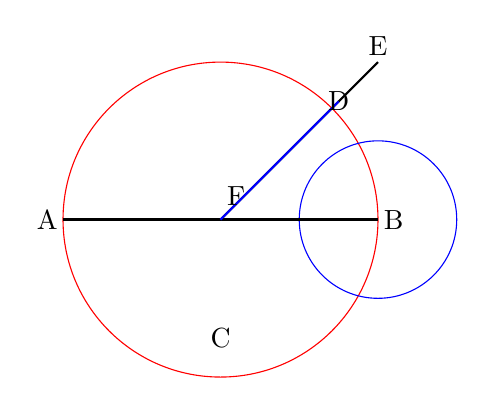
\begin{tikzpicture}
% 绘制圆和直线
\draw[red] (0,0) circle(2); % 外圆
\draw[blue] (2,0) circle(1); % 内圆
\draw[black, thick] (-2, 0) -- (2, 0); % AB
\draw[black, thick] (0, 0) -- (1.5, 1.5); % AC
\draw[black, thick] (1.5, 1.5) -- (2, 2); % CD
\draw[blue, thick] (1.5, 1.5) -- (0, 0); % AE

% 标记点
\node at (-2.2, 0) {A};
\node at (2.2, 0) {B};
\node at (0, -1.5) {C};
\node at (1.5, 1.5) {D};
\node at (2, 2.2) {E};
\node at (0.2, 0.3) {F};

\end{tikzpicture}

\end{document}
